\section{PyNEMO 3: Aplicaci\'on con algoritmos de busqueda.}

\textbf{PyNemo 3} es una aplicaci\'on escrita en Python \cite{wiki:python} como se muestra en la Figura \ref{fig:gui} que permite cargar un archivo de texto que contiene un escenario desde un archivo de texto plano con un formato como el que se especifica en la anterior secci\'on.
\begin{figure}[!h]
	\centering
	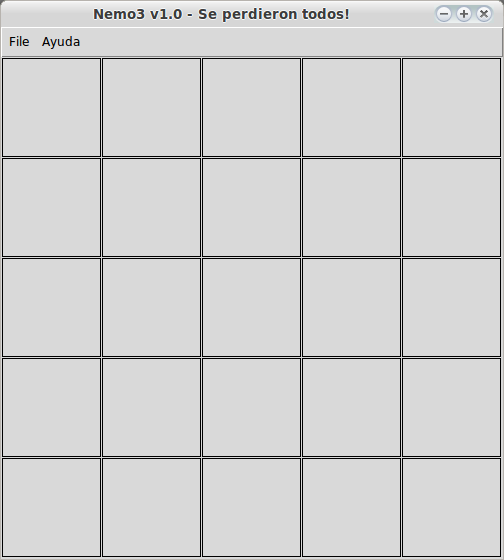
\includegraphics[width=0.3\textwidth]{gui.png}
	\caption{Interfaz grafica (GUI) de Nemo3}
	\label{fig:gui}
\end{figure}

Una vez cargado un archivo de texto este pinta un ambiente con colores que representan cada uno de los elementos especificados en el archivo y que representan el escenario de ejecuci\'on, para la entrada especificada en la \ref{fig:entrada} la interfaz gr\'afica quedara como \ref{fig:entradagui}
\begin{figure}[!h]
	\centering
	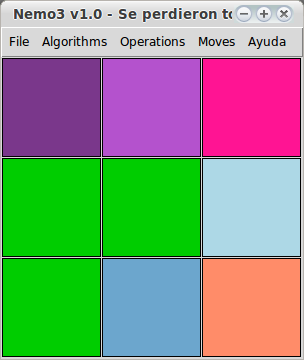
\includegraphics[width=0.3\textwidth]{entradagui.png}
	\caption{Interfaz grafica (GUI) de Nemo3}
	\label{fig:entradagui}
\end{figure}

La representaci\'on de colores que utiliza \textbf{PyNemo 3} se encuentra en un cuadro de dialogo que puede ser abierto desde el men\'u ayuda \ref{fig:ayuda}
\begin{figure}[!h]
	\centering
	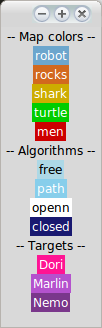
\includegraphics[width=0.1\textwidth]{ayuda.png}
	\caption{Ayuda de la Interfaz grafica (GUI) de Nemo3}
	\label{fig:ayuda}
\end{figure}

Este men\'u de ayuda indica los colores que se encuentran en el mapa, los elementos que puede modificarse con el algoritmo y los objetivos.
Esta aplicaci\'on es orientada a objetos, y por tal raz\'on un algoritmo se trata como una instancia en un hilo que puede ser detenida, ralentizada o acelerada durante la ejecuci\'on, cada uno de los algoritmos implementados, puede leer ambiente, que posee varias colecciones de acuerdo a lo que se ha encontrado en el archivo de texto.

De acuerdo con lo anterior \textbf{PyNemo 3} permite seleccionar la estrategia que el usuario final desea ejecutar en el ambiente cargado, el orden de los movimientos que desea que el algoritmo tenga en cuenta (operadores), adem\'as un conjunto de operaciones como iniciar la ejecuci\'on, detener la ejecuci\'on, hacer la transici\'on de estados, abiertos y cerrados lento o r\'apido y limpiar los cambios que ha hecho el algoritmo en la interfaz.

Una vez termine la ejecuci\'on del algoritmo se pinta la ruta que ha encontrado, además permite guardar en un archivo de texto la salida de la ejecuci\'on.\\\\
\textbf{Pasos soluc\'ion:} \( (X,Y)->(X,Y)->...->(X,Y) \)\\
\textbf{Nodos expandidos:} X \\
\textbf{Nodos creados:} Y \\
\textbf{Costo total soluci\'on:} Z \\
\textbf{Factor ramificaci\'on:} W 

La puesta en marcha realiza con el comando \textit{python nemo3.py}, la interfaz esta construida con Tkinter y con python2.7 que deben estar instalados en el computador que se desea ejecutar la aplicaci\'on
